\part{Background and Problem Identification}

\chapter{Introduction}\label{chap:introduction}
\myquote{Finding Quotes for Dissertation Chapters is Procrastination.}{Anonymous}

\baseduponchapter{\cite{Weske2012BusinessProcessManagement}}

\hypothesisChapter{1}{Some Hypothesis text.}

\marginnote{Note}
\lipsum[1]

\section{Context}\label{sec:introduction:context}

\baseduponsection{\cite{Weske2012BusinessProcessManagement}}

\hypothesisSection{1}{Some Hypothesis text.}

\marginnote{Note}
\lipsum[2]

\patternOneDefinition

\marginnote{Note}
\lipsum[3]

\definitionown{Term}{A term is a word that defines something specific.}

\marginnote{Note}
\lipsum[4]

\definitioncited{\acl{BPM}}{Business process management includes concepts, methods, and techniques to support the design, administration, configuration, enactment, and analysis of business processes.}{\cite[p.~5]{Weske2012BusinessProcessManagement}}

\marginnote{Note}
\lipsum[5]

\hypothesisDefinition{1}{Some Hypothesis text.}

\marginnote{Note}
\lipsum[6]

\marginnote{Note}
\lipsum[7]

Again some\footnote{\url{www.jabref.org} \lastaccessed} words.

\marginnote{Note}
\lipsum[8]

\pattern{Name}{Problem}{Solution}{Example}{Relations to other Patterns}

\marginnote{Note}
\lipsum[9]

\section{Problem Statement}

\marginnote{Note}
\lipsum[9]

We refer to \patternOneReference as this is an important pattern. It really is. Trust us. Don't think for yourself. Just trust us.

\marginnote{Note}
\lipsum[10]

\begin{mdframed}[backgroundcolor=black!20,rightline=false,leftline=false,topline=false,bottomline=false]
\begin{description}
\item[\textbf{User Story Name}:]\userstory{child}{get my own TV}{watch TV whenever I want}
\end{description}
\end{mdframed}

\marginnote{Note}
\lipsum[11]

\begin{figure}[htb]
\centering
\footnotesize
\caption{Example File System Tree}\label{fig:example-file-system-tree}
\framebox[\textwidth]{%
\begin{minipage}{0.9\textwidth}
\dirtree{%
.1 my-passwords$.$txt.
.1 stolen/.
.2 passwords/.
.3 other-passwords$.$txt.
}
\end{minipage}
}
\end{figure}

\marginnote{Note}
\lipsum[12]

\begin{pseudoCode}{Pseudo Code of the Loader Algorithm}{lst:pebash:loader}
def solve(problem):
    analyze problem
    check problem
    solve it
\end{pseudoCode}

\marginnote{Note}
\lipsum[13]

\begin{xmlCode}{This is XML}{lst:xml-code}
<node>
    <!-- comment (use 4 spaces for indent, no tabs) -->
    <element attribute="true" ... />
</node>
\end{xmlCode}

\marginnote{Note}
\lipsum[13]

\begin{figure}[htb]
\centering
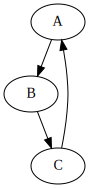
\includegraphics[width=4cm]{figures/example}
\caption{Some Example Figure generated from GRAPHVIZ DOT}\label{fig:intro:example}
\end{figure}

\marginnote{Note}
\lipsum[14]

\begin{figure}[htb]
\centering
\includegraphics[width=\linewidth]{figures/example-pptx-figure}
\caption{Some Example Figure generated from a single PPTX Slide}\label{fig:intro:example2}
\end{figure}

\marginnote{Note}
\lipsum[15]